\documentclass{article}

\usepackage[english]{babel}
\usepackage[utf8]{inputenc}
\usepackage{amsmath}
\usepackage{amsthm}
\usepackage{amssymb}
\usepackage{mathtools}
\usepackage{amsfonts}
\usepackage{subcaption}
\usepackage{graphicx}
\usepackage{wrapfig}
\usepackage{bbm}
\usepackage{dsfont}
\usepackage{listings}

% set up margin
\usepackage
[
  a4paper,
  left=3cm,
  right=3cm,
  top=3cm,
  bottom=3cm,
]
{geometry}

% set up header
\usepackage{fancyhdr}
\pagestyle{fancy}
\fancyhf{}
\lhead{6.438 Algorithms for Inference}
\chead{Problem Set 4}
\rhead{Hongzi Mao}
\cfoot{\thepage}
\rfoot{\footnotesize{\emph{Collaborated with: Hongzhou Ye, Zhiwei Ding}}}

% footer line
\renewcommand{\footrulewidth}{0.4pt}

% sans serif italic
\newcommand{\s}[1]{\textsf{\textit{#1}}}

% bold face sans serif
\newcommand{\bs}[1]{\textsf{\textbf{#1}}}

% set symbol
\usepackage[mathscr]{euscript}

% empty set
\let\emptyset\varnothing

% qed
\newcommand{\qeds}{\hfill\qedsymbol}

% math bold face
\newcommand{\bm}{\mathbf}

% argmax
\DeclareMathOperator*{\argmax}{argmax}
\DeclareMathOperator*{\argmin}{argmin}

% colorful reference
\usepackage{hyperref}
\usepackage{color}
\definecolor{darkred}{rgb}{0.7,0,0}
\definecolor{darkgreen}{rgb}{0,0.5,0}
\hypersetup{colorlinks=true,
        linkcolor=darkred,
        citecolor=darkgreen}
\urlstyle{same}

% independence symbol
\makeatletter
\newcommand*{\indep}{%
  \mathbin{%
    \mathpalette{\@indep}{}%
  }%
}
\newcommand*{\nindep}{%
  \mathbin{%                   % The final symbol is a binary math operator
    \mathpalette{\@indep}{\not}% \mathpalette helps for the adaptation
                               % of the symbol to the different math styles.
  }%
}
\newcommand*{\@indep}[2]{%
  \sbox0{$#1\perp\m@th$}%        box 0 contains \perp symbol
  \sbox2{$#1=$}%                 box 2 for the height of =
  \sbox4{$#1\vcenter{}$}%        box 4 for the height of the math axis
  \rlap{\copy0}%                 first \perp
  \dimen@=\dimexpr\ht2-\ht4-.2pt\relax
  \kern\dimen@
  {#2}
  \kern\dimen@
  \copy0 %                       second \perp
} 
\makeatother

%%%%%%%%%%%%%%%%%%%%%%%%%%%%%%%%%%%%%%%%%%%%%%%%%%%%%%%%%%%%%%%%%%%%%%%%
%%%%%%%%%%%%%%%%%%%%%%%%% Begin document here %%%%%%%%%%%%%%%%%%%%%%%%%%
%%%%%%%%%%%%%%%%%%%%%%%%%%%%%%%%%%%%%%%%%%%%%%%%%%%%%%%%%%%%%%%%%%%%%%%%
\begin{document}

\section*{Problem 5.1}
%
(a) We check local consistency by checking the marginals sum to 1 and the
edge marginals marginalize to node marginal. That is
%
\begin{align*}
	b_i(0) + b_i(1) = 0.5 + 0.5 = 1,
\end{align*}
%
for $\forall i \in \{1, 2, 3\}$; and
\begin{align*}
	b_{ij}(0,0) + b_{ij}(0,1) + b_{ij}(1,0) + b_{ij}(1,1) = 1,
\end{align*}
%
for $\forall i, j \in \{1, 2, 3\}, i \neq j$;
and\footnote{$b_i(1)$ checks out similarly for $\forall \{1,2,3\}$}
%
\begin{align*}
	b_{12}(0, 0) + b_{12}(0, 1) = 0.49 + 0.01 = 0.5 &= b_1(0),\\
	b_{12}(1, 0) + b_{12}(0, 0) = 0.01 + 0.49 = 0.5 &= b_2(0),\\
	b_{32}(0, 0) + b_{32}(0, 1) = 0.49 + 0.01 = 0.5 &= b_3(0),\\
	b_{32}(1, 0) + b_{32}(0, 0) = 0.01 + 0.49 = 0.5 &= b_2(0),\\
	b_{31}(0, 0) + b_{31}(0, 1) = 0.01 + 0.49 = 0.5 &= b_3(0),\\
	b_{31}(1, 0) + b_{31}(0, 0) = 0.49 + 0.01 = 0.5 &= b_1(0).\\
\end{align*} \qeds
%
\\

\noindent
(b) We prove this by contradiction. Suppose such distribution
$p_{\s{x}_1, \s{x}_2, \s{x}_3}(x_1, x_2, x_3)$ exists, then
\begin{align}
	&p_{\s{x}_1, \s{x}_2, \s{x}_3}(0, 0, 0) + p_{\s{x}_1, \s{x}_2, \s{x}_3}(0, 0, 1) = b_{12}(0, 0) = 0.49, \label{51b1}\\
	&p_{\s{x}_1, \s{x}_2, \s{x}_3}(0, 0, 0) + p_{\s{x}_1, \s{x}_2, \s{x}_3}(0, 1, 0) = b_{31}(0, 0) = 0.01, \label{51b2}\\
	&p_{\s{x}_1, \s{x}_2, \s{x}_3}(0, 0, 1) + p_{\s{x}_1, \s{x}_2, \s{x}_3}(1, 0, 1) = b_{32}(0, 1) = 0.01. \label{51b3}
\end{align}
%
Since we assume $p_{\s{x}_1, \s{x}_2, \s{x}_3}(\cdot)$ is a valid distribution, we have
\begin{align*}
	p_{\s{x}_1, \s{x}_2, \s{x}_3}(x_1, x_2, x_3) \geq 0,
\end{align*}
for $\forall (x_1, x_2, x_3) \in \{0, 1\}^3$.

Now, from Equation~\eqref{51b2}, we have
\begin{align*}
	p_{\s{x}_1, \s{x}_2, \s{x}_3}(0, 0, 0) \leq 0.01,
\end{align*}
from from Equation~\eqref{51b3}, we have
\begin{align*}
	p_{\s{x}_1, \s{x}_2, \s{x}_3}(0, 0, 1) \leq 0.01.
\end{align*}
%
Thus, 
\begin{align*}
	p_{\s{x}_1, \s{x}_2, \s{x}_3}(0, 0, 0) + p_{\s{x}_1, \s{x}_2, \s{x}_3}(0, 0, 1) \leq 0.01 + 0.01 = 0.02,
\end{align*}
%
which contradicts with Equation~\eqref{51b1}, where 
$p_{\s{x}_1, \s{x}_2, \s{x}_3}(0, 0, 0) + p_{\s{x}_1, \s{x}_2, \s{x}_3}(0, 0, 1) = 0.49$.
\qeds
\\
\\
\\
\\
\\
\\
\\
\\
\\
\\

\pagebreak
%
%%%%%%%%%%%%%%%%%%%%%%%%%%%%%%%%%%%%%%%%%%%%%%%%%%%%%%%%%%%%%%%%%%%%%%%% 
\section*{Problem 5.2}
(a) With slight abuse of notations, we index the node with the coordinate
$(i, j)$ in the image. Figure~\ref{f:52a} sketches the undirected graphs.
%
\begin{figure}[h]
  \centering
  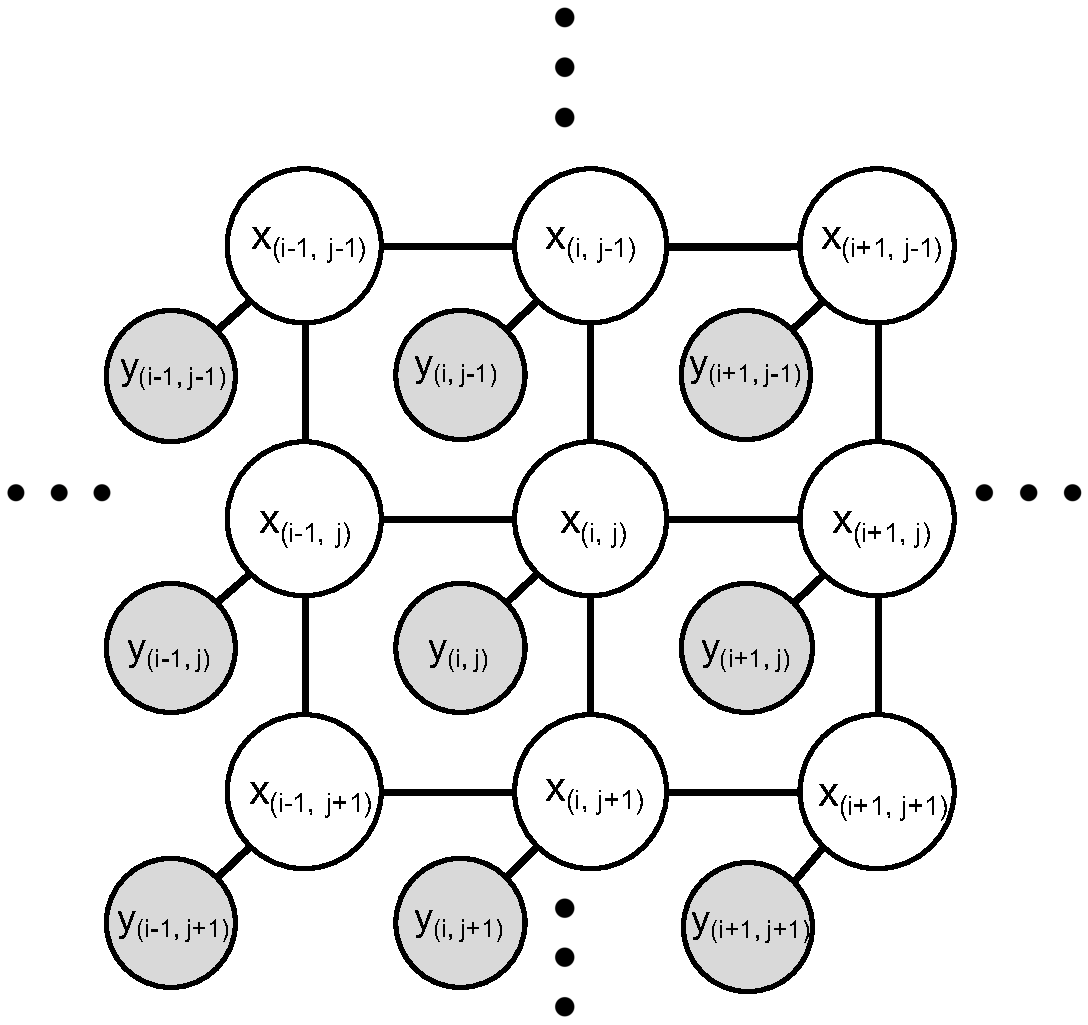
\includegraphics[width=0.4\columnwidth]{52a.pdf}
    \vspace{-0.1cm}
  \caption{Undirected graph of the 5.2 photography problem.}
  \label{f:52a}
\end{figure}
%

The potential function $\psi(x_i, y_i)$ is given by
\begin{align*}
	\psi(x_i, y_i) = \frac{1}{(2\pi)^{3/2}(\det {\bf\Lambda}_{x_i})^{1/2}}
	\exp\left[-\frac{1}{2}(y_i-\mu_{x_i})^T\mathbf{\Lambda}^{-1}_{x_i}(y_i - \mu_{x_i})\right] + \epsilon.
\end{align*}
\\

\noindent
(b) For the labeled masks, we empirically compute
\begin{align*}
	&\mu_\alpha = \frac{1}{N_\alpha}\sum_{i=1}^{N_\alpha}y_i,\\
	&\mathbf{\Lambda}_{\alpha} = \frac{1}{N_\alpha}\sum_{i=1}^{N_\alpha}\left[(y_i - \mu_\alpha)(y_i - \mu_\alpha)^T\right],
\end{align*}
where $N_\alpha$ is the number of pixels in the labeled mask.
%

In the \texttt{flower} example, we have for the foreground
\begin{align*}
	\mu_1 = 
	\begin{bmatrix}
    168.29 \\
    95.19 \\
    8.48
\end{bmatrix}, \;\;\,
	\mathbf{\Lambda}_1 =
\begin{bmatrix}
 94.89 & 122.81 & 144.93 \\
 122.81 & 111.90 & 105.58 \\
 144.93 & 105.58 &  68.92
\end{bmatrix},
\end{align*}
and the background
\begin{align*}
	\mu_0 = 
	\begin{bmatrix}
    78.79 \\
    79.10 \\
    41.24
\end{bmatrix}, \;\;\,
	\mathbf{\Lambda}_0 =
\begin{bmatrix}
104.27 & 133.14 & 130.03 \\
133.14 & 106.70 & 121.70 \\
130.03 & 121.70 & 102.89
\end{bmatrix}.
\end{align*}
The code for this computation is attached in the bottom.
\\

\noindent
(c)
We denote the indices of the neighboring pixels of $j$ as $\partial j$. That is the observation $y_j$ is not a member of $\partial j$ and we consider the message from it separately. The update rule for the message passing is
\begin{align*}
	m_{j\to k}(x_k) &= \sum_{x_j} \psi_{jk}(x_j, x_k)\,\,m_{y_j\to x_j}(x_j) \prod_{l\in\partial{j}\backslash\{k\}}m_{l\to j}(x_j)\\
	&\propto \sum_{x_j} \big[0.9\times\mathds{1}_{x_j = x_k} + 0.1\times\mathds{1}_{x_j \neq x_k} \big] \times\\
	& \left\{\frac{1}{(2\pi)^{3/2}(\det {\bf\Lambda}_{x_j})^{1/2}} \exp\left[-\frac{1}{2}(y_j-\mu_{x_j})^T\mathbf{\Lambda}^{-1}_{x_j}(y_j - \mu_{x_j})\right] + \epsilon\right\}
	\times \prod_{l\in\partial{j}\backslash\{k\}}m_{l\to j}(x_j).
\end{align*}
%

To compute the marginal, the final belief update rule on $x_i$ is
\begin{align*}
	p_{\s{x}_i}(x_i) &\propto  m_{y_i\to x_i}(x_i) \prod_{j\in\partial{i}}m_{j\to i}(x_i)\\
	&\propto \left\{\frac{1}{(2\pi)^{3/2}(\det {\bf\Lambda}_{x_i})^{1/2}} \exp\left[-\frac{1}{2}(y_i-\mu_{x_i})^T\mathbf{\Lambda}^{-1}_{x_i}(y_i - \mu_{x_i})\right] + \epsilon\right\}
	\times \prod_{j\in\partial{i}}m_{j\to i}(x_i).
\end{align*}
\\

\noindent
(d)




\end{document}